
\startslide{Outline}
\begin{cenumerate}
\item Motivation, overview
\item Technical details
\begin{citemize}
\item Language design 
\item Formal foundations
\end{citemize}
\item Language implementation and application
\end{cenumerate}
\stopslide

%%%%%

\startslide{The Problem Setting: Embedded Sensor Networks}
\begin{center}
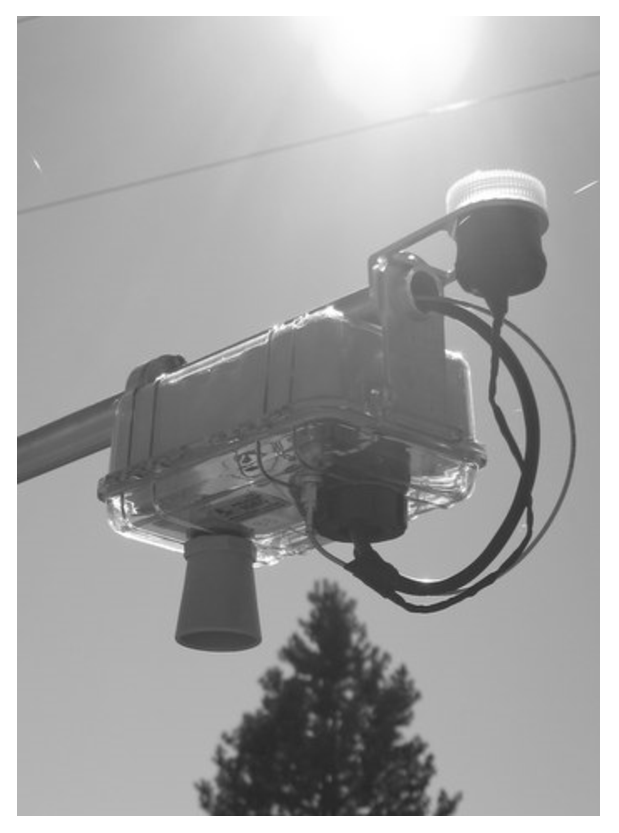
\includegraphics[scale=.50]{brainbox} 
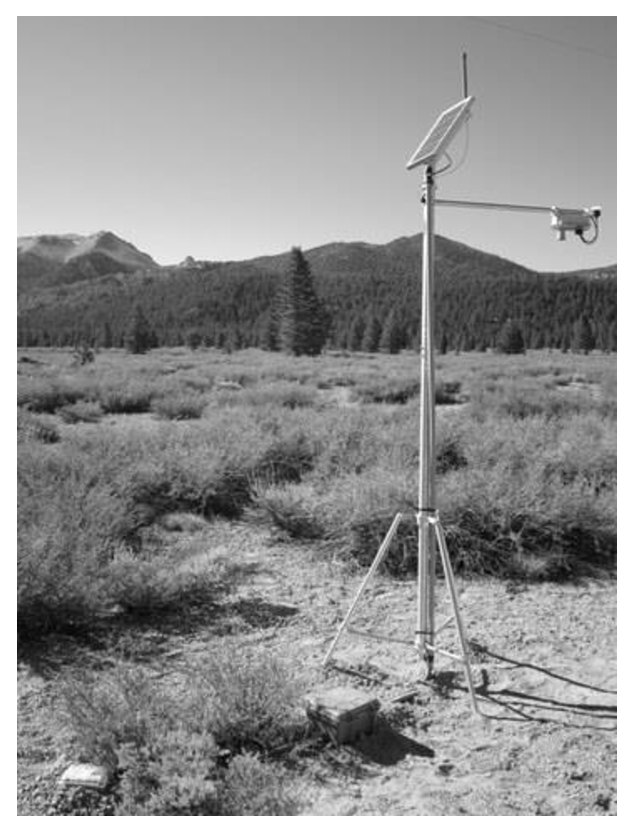
\includegraphics[scale=.50]{tower} 
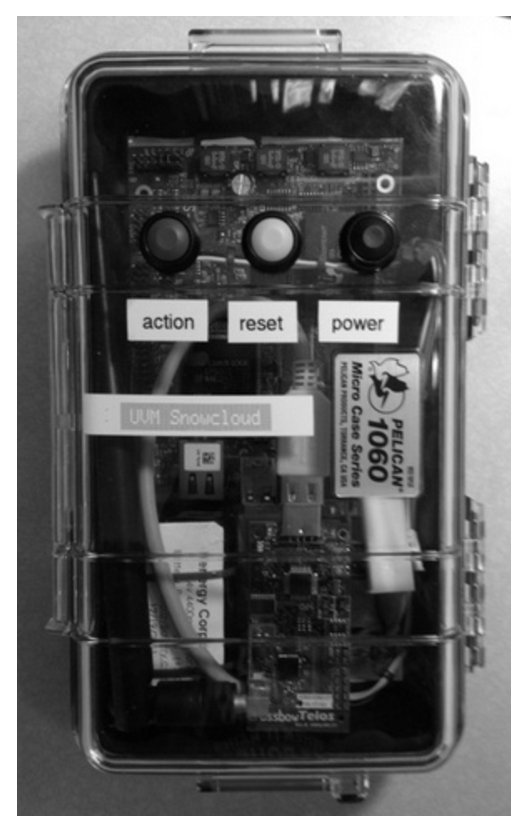
\includegraphics[scale=.50]{harvester} 
\end{center}

\begin{citemize}
\item Distributed data-gathering systems for earth and agricultural sciences.
\item At UVM, focus on alpine snow hydrology.
\begin{citemize}
\item Deployments in California, New Hampshire, Arctic Norway.
\end{citemize}
\end{citemize}
\stopslide

%%%%%

\startslide{Challenges of Programming Sensor Networks}
\begin{citemize}
\item Heavily resource constrained---RAM, ROM, clock cycles, power.
\item E.g., Crossbow TelosB: 4\,MHz, 10\,KiB RAM, 48\,KiB ROM
\item \ldots yet complex, distributed algorithms used
\end{citemize}

State of the art:
\begin{citemize}
\item NesC and TinyOS: optimized for efficiency, widely used.
\item Various \cemph{macroprogramming} proposals, but mostly ad hoc node level programming
  techniques in practice.
\end{citemize}
\stopslide

%%%%%

\startslide{Staging as a Tool}
In the lab:
\begin{citemize}
\item Create first stage program to specialize and compose modules of second stage code.
\end{citemize}

In the field on a base station or \cemph{hub}:
\begin{citemize}
\item Execute first stage program to generate second stage program accounting for field
  conditions.
\item Deploy second stage program to nodes (over the air).
\end{citemize}
\stopslide

%%%%%

\startslide{Workflow}
\hspace*{.6in}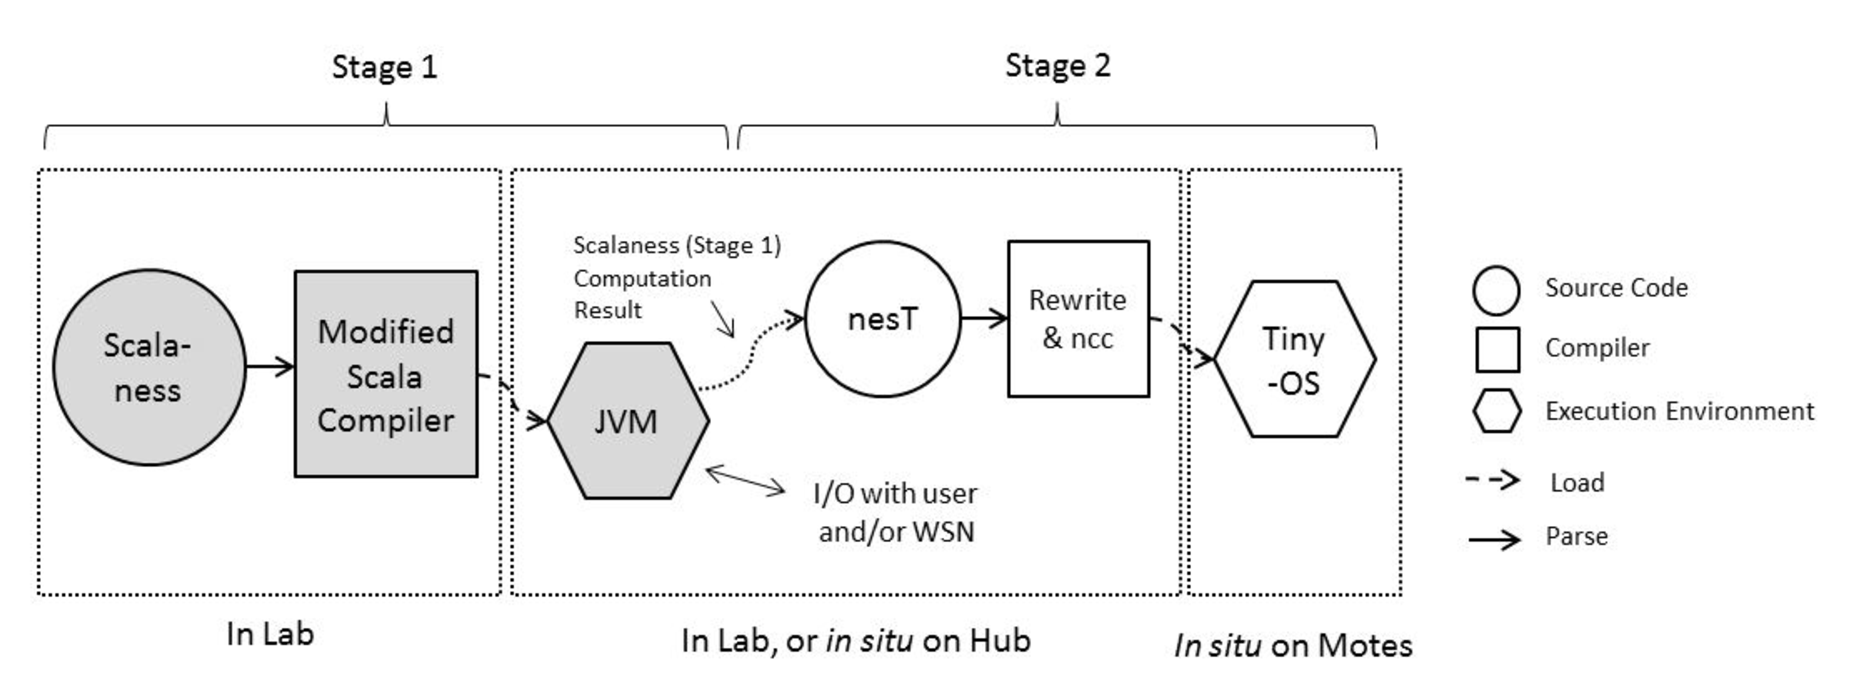
\includegraphics{scalaness}
\stopslide

%%%%%

\startslide{Our Approach}
\begin{citemize}
\item \cemph{Lightweight macroprogramming}. Scala at metalevel, nesC residuum.
\item Technical features: type specialization, process separation.
\item \cemph{Cross-stage type safety}: type checking at Scala level ensures type safety of nesC
  residuum.
\item \cemph{Well-founded language design}.
\end{citemize}
\stopslide

%%%%%

\startslide{Presentation Outline}
\begin{cenumerate}
\item Motivations, design overview
\item \cemph{Technical details}
\begin{citemize}
\item \cemph{Language design} 
\item Formal foundations
\end{citemize}
\item Language implementation and application
\end{cenumerate}
\stopslide

%%%%%

\startslide{Example: Introducing Some Type Abbreviations}
\lstset{basicstyle=\ttfamily, escapeinside={(*@}{@*)}}
\begin{lstlisting}
(*@\tt{abbrvt\ mesgT(t) =}@*)
  { src : (*@\tt{t}@*); dest : (*@\tt{t}@*); data : uint8[] };

(*@\tt{abbrvt\ radioT =}@*)
  < at (*@$\subtype$@*) uint >
  { export error_t radio_x((*@\tt{mesgT}@*)(at)*); 
    import error_t handle_radio_r((*@\tt{mesgT}@*)(at)*); };

(*@\tt{abbrvt\ commT =}@*)
  (at (*@$\subtype$@*) uint) (*@$\circ$@*) < >
  { export error_t send((*@\tt{mesgT}@*)(at)*); 
    import error_t handle_receive((*@\tt{mesgT}@*)(at)*); };
\end{lstlisting}
\stopslide

%%%%%

\startslide{Example: DnesT Modules}
\lstset{basicstyle=\ttfamily, escapeinside={(*@}{@*)}}
\begin{lstlisting}
(*@\tt{authSend =}@*)
  < at (*@$\subtype$@*) uint; sendk : uint8[] >  
  { import error_t radio_x((*@\tt{mesgT}@*)(at)*);
    export error_t send(m : (*@\tt{mesgT}@*)(at)*) 
        { radio_x(AES_sign(m, sendk)); }
  };

(*@\tt{authRecv =}@*)
  < at (*@$\subtype$@*) uint; recvk : uint8[] >  
  { import error_t handle_recv((*@\tt{mesgT}@*)(at)*);
    export error_t handle_radio_r(m : (*@\tt{mesgT}@*)(at)*) 
        { if AES_signed(m, recvk) 
              handle_recv(m); }
  };
\end{lstlisting}
\stopslide

%%%%%

\startslide{Example: DScalaness Method}
\lstset{basicstyle=\ttfamily, escapeinside={(*@}{@*)}}
\begin{lstlisting}
def authSpecialize
 (nmax   : uint16,
  radioM : radioT,
  keys   : Array[Array[uint8]]) : commT {

    typedef adt (*@$\subtype$@*) uint =
      if (nmax <= 256) uint8 else uint16;

    val sendM = (*@\jinst{authSend}{adt; keys(0)}@*);
    val recvM = (*@\jinst{authRecv}{adt; keys(1)}@*);
    sendM (*@$\ltimes$@*) (*@\jinst{radioM}{adt}@*) (*@$\ltimes$@*) recvM;
}
\end{lstlisting}
\stopslide

%%%%%

\startslide{Example: Generating nesT (and nesC)}
\lstset{basicstyle=\ttfamily, escapeinside={(*@}{@*)}}
\begin{lstlisting}
 (*@\tt{appMR\ =}@*) 
  < >
  { export handle_recv(m : (*@\tt{mesgT}@*)(uint8)*) {(*@\ldots@*)} }; 

 (*@\tt{appM\ =}@*) 
  < >
  { import send((*@\tt{mesgT}@*)(uint8)*); export main() {(*@\ldots@*)} };  

 image(appM (*@$\ltimes$@*)
         authSpecialize(nmax, radioM, keys) (*@$\ltimes$@*)
           appMR);
\end{lstlisting}
\stopslide

%%%%%

\startslide{Presentation Outline}
\begin{cenumerate}
\item Motivations, design overview
\item \cemph{Technical details}
\begin{citemize}
\item Language design 
\item \cemph{Formal foundations}
\end{citemize}
\item Language implementation and application
\end{cenumerate}
\stopslide

%%%%%

\startslide{\fml\ Foundations}
The \fml\ language\footnote{\cref{Yu David Liu, Christian Skalka, and Scott Smith. Type-Specialized Staged Programming with Process Separation. Journal of Higher Order and Symbolic Computation, 24(4):341-385, 2012.}} was developed to study these elements at a foundational level.
\begin{citemize}
\item Comprises $F_{\le}$.
\item MetaML-like syntax and semantics, but novel features to moderate 
interactions between separate process spaces.
\item Resricted form of type construction (not full $\lambda_\omega$).
\item Formal metatheory includes cross-stage type safety-- residue of  
partial evaluation of well-typed code is guaranteed to be well-typed.
\end{citemize}
\stopslide

%%%%%

\startslide{The Model of a Module}
The essence of a nesT module definition:
{\Large
$$
\lambda x : \tau_1 . \Lambda t \subtype \tau_2 . \langle e \rangle
$$
}
\begin{citemize}
\item $\langle e \rangle$ is code-as-value (the ``module definition'').
\item $\lambda$ binds ``value parameter''.
\item $\Lambda$ binds ``type parameter'', with type bound.
\item If $x$ is free in $e$, then $\tau_1 = \langle \tau \rangle$. \cemph{The stage levels must match}.
\end{citemize}
\stopslide

%%%%%

\startslide{The Model of Module Instantiation}
The essence of a Scalaness/nesT module instantiation:
{\Large
$$
(\lambda x : \tau_1 . \Lambda t \subtype \tau_2 . \langle e \rangle)(\mathrm{lift}\ v) \tau
$$
}
\begin{citemize}
\item Value $v$ must be explicitly ``lifted'' to next stage.
\begin{citemize}
\item Only way for values to migrate across stages, no free variable capture as in 
MetaML.
\item Lifting enforces serialization (implicit lifting in Scalaness).
\item Enforced by the type system: require that $\tau_1 = 
\langle \tau' \rangle$ and $v : \tau'$.
\end{citemize}
\end{citemize}
\stopslide

%%%%%

\startslide{Type Construction and Escape}
A $\mathrm{tlet}$ binding mechanism allows construction of types:
{\large
$$
\mathrm{tlet\ } t \subtype \mathrm{uint16} = \metaite{e}{\mathrm{uint8}}{\mathrm{uint16}} 
\mathrm{\ in\ }(\lambda x : t . x)\\
$$
}
\begin{citemize}
\item Restriction: only concrete types are values, no higher-order type constructors.
\item Dynamically constructed types may escape their scope.
\end{citemize}
\stopslide

%%%%%

\startslide{Type Construction and Escape}
We introduce an \cemph{$\exists$ type binder} for typing constructed type escape:
{\large
\begin{eqnarray*}
&\mathrm{tlet\ } t \subtype \mathrm{uint16} = \metaite{e}{\mathrm{uint8}}{\mathrm{uint16}} 
\mathrm{\ in\ }(\lambda x : t . x)\\
&: \\
&\exists t \subtype \mathrm{uint16} . t \rightarrow t
\end{eqnarray*}
}
\cemph{Execution obtains a \emph{refinement} of the type}; assuming $e \rightarrow^* \mathrm{true}$:
{\large
$$
\ldots \rightarrow^* (\lambda x : \mathrm{uint8} . x) 
\qquad \text{where} \ \ (\lambda x : \mathrm{uint8} . x) : \mathrm{uint8} \rightarrow
 \mathrm{uint8}
$$
}
Cross-stage type safety does not interfere with code type specialization.
\stopslide

%%%%%

\startslide{$\exists$ Type?}
Usage of $\exists$ type is non-standard.
\begin{citemize}
\item No pack, unpack rules.
\end{citemize}
But several appealing features of the approach:
\begin{citemize}
\item Sound typing $\Gamma, \Delta \vdash e : \tau$ must \cemph{encapsulate} the definition of constructed types.

{\small
\begin{mathpar}
\inferrule[TLet]
{
\stjudge{\Gamma}{\Delta}{e}{\typet[\sigma]}\\
%\Delta \vdash \tau'' \subtype \tau'\\
\stjudge{\Gamma}{\Delta; t \subtype \sigma}{e'}{\tau}
}
{\stjudge{\Gamma}{\Delta}{\tlet{t \subtype \sigma}{e}{e'}}
  {\exists t \subtype \sigma . \tau}}

\inferrule[$\exists$-E]{\Gamma, \Delta; \vdash e : \exists t \subtype \tau' . \tau
  \\  t \not\in \Delta, \Gamma}{
 \Gamma, \Delta; t\subtype \tau' \vdash e : \tau}
\end{mathpar}
}

where $\Delta$ subtyping coercions, $\Gamma$ free variable typings, $t$ in \TirName{TLet}
has \emph{eigenvariable} interpretation.
\end{citemize}
\stopslide

%%%%%

\startslide{$\exists$ Type?}
Bounded $\exists$ type form well-studied, esp.~Ghelli and Pierce 1998:
\begin{citemize}
\item Crucial elements of type checking in $F_\le$ (\emph{promotion}).
\item \cemph{Decidable} subtyping relation, with algorithm.
\begin{citemize}
 \item Covariant $\exists$ type bounds sound but undecidable.
 \item Invariant $\exists$ bounds decidable. 
\end{citemize}
\end{citemize}
\stopslide

%%%%%

\startslide{Putting it together in Scalaness}
$$
\jmodt{\Delta_1}{\margs{\Delta_2, \Gamma}\lc 
  \imports; \exportsty \rc}
$$
Module type form, where:
\begin{citemize}
\item $\Delta_1$ bounds of types constructed externally to the module
\item $\Delta_2$, $\Gamma$ type parameter bounds and term parameter types
\item $\imports$, $\exports$ import and export type signatures
\end{citemize}
$$
\inferrule[ModInstT]
{\Gamma \vdash \tt{e} : \jmodt{\varnothing}{\margs{\vect{t} \subtype \vect{\t}_1; 
 \vect{x} : \vect{\t}_2} \lc 
  \imports; \exportsty \rc}\\
 \Gamma \vdash \ttvec{e}_1 : \jinst{Type}{\ttvec{T}_1}\\
 \Gamma \vdash \ttvec{e}_2 : \ttvec{T}_2 \\
 \vdash \codt{\ttvec{T}_1} \subtype \vect{\t}_1\\
 \vdash \codt{\ttvec{T}_2} \subtype \vect{\t}_2
}
{\Gamma \vdash \jinst{e}{\ttvec{e}_1; \ttvec{e}_2} : \jmodt{\vect{t}\subtype \codt{\ttvec{T}_1}}{\margs{} \lc
  \imports; \exportsty \rc} }
$$

$\codt{T}$ is syntactic type transformation/interpretation (Scalaness to nesT).
\stopslide

%%%%%

\startslide{Presentation Outline}
\begin{cenumerate}
\item Motivations, design overview
\item Technical details
\begin{citemize}
\item Language design 
\item Formal foundations
\end{citemize}
\item \cemph{Language implementation and application}
\end{cenumerate}
\stopslide

%%%%%

\startslide{Implementation}
Scalaness/nesT has been implemented.
\begin{citemize}
\item nesT defined as restricted subset of nesC, compiled as nesC with some 
rewriting (e.g.~array bounds checks).
\item Scalaness defined by extension to the Scala compiler and plugin architecture.
\item Type checking extends Scala type checker with module types, module operation 
typings, nesT type checking. 
\end{citemize}
Github repository at \url{http://tinyurl.com/a85z8cu}.
\stopslide

%%%%%

\startslide{Application: WSN Session Key Negotiation}
Currently studying authorization scheme for WSNs.
\begin{citemize}
\item WSN may comprise interacting security domains with different credentials
and policies.
\item Symmetric keys provide efficient foundation for securing access.
\item Public keys allow symmetric key negotiation (Diffie-Hellman) in ``open world''
model.
\end{citemize}
Public key signature verification wildly expensive in WSNs; around 90 seconds
on Crossbow TelosB.

\cemph{Refactor session key negotiation and authorized access into 
different stages.}
\stopslide

%%%%%

%\startslide{Application: WSN Session Key Negotiation}
%
%Use Scalaness/nesT to orchestrate more efficient key negotiation:
%\begin{citemize}
%\item 
%\item Key negotiation performed over on communicating high-powered 
%hubs in first stage code.
%\item Specialize second stage code with negotiated key material, deploy 
%to WSN nodes for authorized resource access.
%\end{citemize}
%\stopslide

%%%%%

\startslide{Application: WSN Session Key Negotiation}
\hspace*{.6in}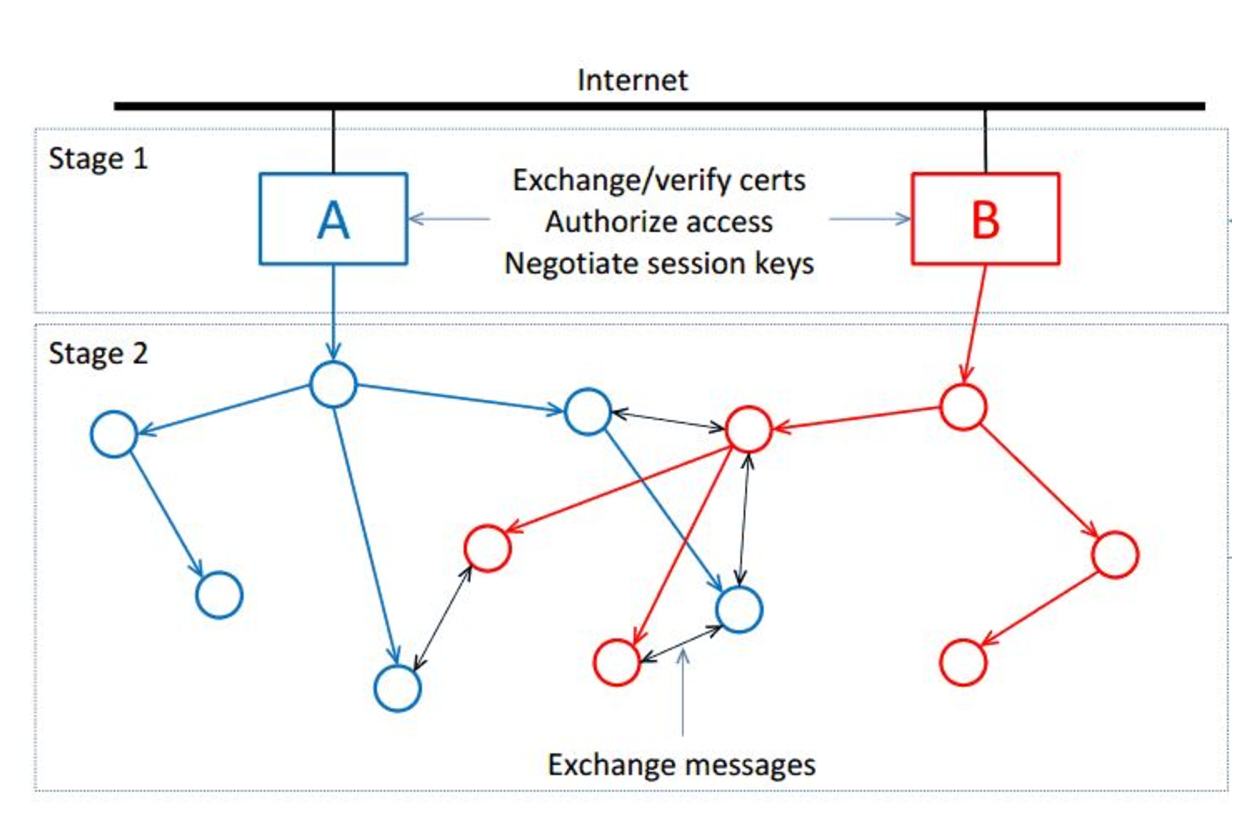
\includegraphics{spartanrpc}

Decreases WSN computational overhead, RAM and ROM consumption. 
\stopslide

%%%%%

\startslide{Future Work}
\begin{citemize}
\item Clarifying ``middle ground'' between langage borders, syntactic transformations.
\item Incorporating network communication. 
\item Other applications: backcasting and evolving control.
\end{citemize}
\stopslide

%%%%%

\startslide{Questions?}
\makeatletter
\center{Peter Chapin \textless pchapin@cs.uvm.edu\textgreater}
\center{Scalaness source: \cemph{https://github.com/pchapin/scala}}
\makeatother
\stopslide
